\section{Recomendación Radares}

\subsection{Métricas y Utilidad}

Este script genera el ``Score de Necesidad de Fiscalización'' y una etiqueta 
prescriptiva de ``Prioridad de Radar''. Mientras que el modelo de puntos 
críticos diagnostica dónde existe peligro, este modelo evalúa la necesidad
de instalar radares de velocidad. Pondera zonas con altas velocidades,
accidentes, y flujo de vehiculos para asignar prioridades (Alta, Media, Baja).

\subsection{Lógica General}

\subsubsection*{Cargar Datos}
Importar el archivo maestro de analítica espacial
(\texttt{tramos\_analitica\_2022.csv}) que contiene las estadísticas 
de tráfico consolidadas por detector.

\subsubsection*{Normalización de Variables}

Extraer las tres variables: velocidad media (\(\mathrm{vel}\)), 
cantidad de accidentes (\(\mathrm{acc}\)) y volumen total
(\(\mathrm{vol}\)).
Luego normalizar estas tres variables dividiendo cada una por su valor 
histórico máximo. 
\begin{align*}
    n_{\mathrm{vel}} &= \operatorname*{norm}(\mathrm{vel}) \\
    n_{\mathrm{acc}} &= \operatorname*{norm}(\mathrm{acc}) \\
    n_{\mathrm{vol}} &= \operatorname*{norm}(\mathrm{vol}) 
\end{align*}

\subsubsection*{Algoritmo de Scoring Ponderado}
Calcular el ``Score de Radar'': 
\begin{align*}
    \mathrm{score} &= 100 \times \left(
        0.4n_{\mathrm{vel}} + 
        0.4n_{\mathrm{acc}} + 
        0.2n_{\mathrm{vol}}
    \right)
\end{align*}
Le damos menos importancia al volumen de autos ya que preferimos prevenir 
velocidades altas y accidentes.

\subsubsection*{Categorización de Prioridades}

Calcular los percentiles estadísticos sobre la distribución de notas 
(scores) de toda la ciudad, esto se hace calculando los cuantiles $q_{n}$ para
delimitar los `mejores' $(100 - n)\%$.

\begin{align*}
    \operatorname*{Prioridad(\mathrm{score})} &= 
    \begin{cases}
        \text{Alta}  & \text{si $\mathrm{score} \geq q_{85}$} \\
        \text{Media} & \text{si $q_{85} > \mathrm{score} \geq q_{50}$} \\
        \text{Baja}  & \text{si $q_{50} > \mathrm{score}$}
    \end{cases}
\end{align*}

\newpage 

\subsection{Reporte}

\begin{figure}[ht]
    \centerline{
        \includegraphics[page=4, scale=0.25]{graphics/reporte.pdf}
    }

    \caption{
        Reporte de las recomendaciones de radares: \\
        (\textbf{izquierda}) Mapa de radares recomendados, de rojo a verde
            indicando prioridad (mayor a menor), y tama\~no de las burbujas 
            indicando \textit{score} calculado. 
        (\textbf{arriba-derecha}) Gr\'afica de embudo, mostrando la cantidad de 
            detectores recomendados. 
        (\textbf{abajo-derecha}) Slider para modificar los detectores mostrados 
            seg\'un el volumen de autos detectados.
    }

    \label{fig:reporte-radares}

\end{figure}
